\chapter{Photon identification and shower shapes}
\label{ch:pid_ss}
\epigraph{\emph{“Champions keep playing until they get it right.”}}{Billie Jean King}

% In \Sect{\ref{subsec:objects:egamma:id}} a very brief description on the identification procedure was described. In the current chapter, a more detailed explanation on the process as well as on the variables used to perform the photon identification is presented. \fixme{elaborate more}

The \ac{ECAL} was presented briefly in \Sect{\ref{subsubsec:atlas:atlas:cals:ecal}}, where the measurement mechanism and all the layers it has was described. In this subdetector, photons deposit their energy via electron-positron pair creation and bremsstrahlung radiation, creating an \ac{EM} shower. The \ac{ECAL} does a great job to compute the energy of the \ac{EM} shower, but identifying the initiating particle remains a challenging task. 
However, by virtue of the different layers and granularities in the \ac{ECAL}, different characteristics of these \ac{EM} showers can be studied, and are encoded by different variables called \acfp{SSV}.

% \fixme{give the overview of the chapter?} As a first step, the variables used to identify correctly the photons are described in detail and the current problem of disagreement between data and \ac{MC} is explained. 






\section{Shower shapes}
\label{sec:pid_ss:ss}

As mentioned in \Sect{\ref{subsec:objects:egamma:id}}, photon identification relies on rectangular cuts applied to \acp{SSV} that lead to an excellent separation power between real isolated photons from fake photons originating from hadrons. These \acp{SSV} are computed from the photon candidates' energy deposits in the \ac{ECAL} and \ac{HCAL} cells, and serve to describe the passage of the photons candidates throughout the calorimeters, characterizing the lateral and longitudinal \ac{EM} showers.

In general, real photons produce narrower energy deposits in the \ac{ECAL}, and have lower leakages to the \ac{HCAL}, compared to those photons proveninent from hadrons, where the presence of additional neighbouring hadrons close to the fake photon tend to widen the showers. Furthermore, since the first layer of the \ac{ECAL} consists on fine strips, it is possible to discriminate photon candidates coming from \(\pizero\to\gamma\gamma\) decays, characterized by two local maxima due to the presence of two nearby photons.

\begin{table}[ht!]
    \caption{Discriminative \acp{SSV} used for photon identification. The three columns on the right denote whether the variable is used for the \textit{loose} (L), \textit{medium} (L) or \textit{tight} (T) identification \ac{WP} or not.}
    \centering
    \resizebox{\textwidth}{!}{
        \begin{tabular}{p{.2\textwidth}p{.50\textwidth}p{0.12\textwidth}|p{.01\textwidth}p{.01\textwidth}p{.01\textwidth}}
            \hline
            \hline
            Category  &  Description  &  Name & L & M & T \\
            \hline
            \hline
            Hadronic leakage
            &  Ratio of \et in the first sampling layer of the \ac{HCAL} to \et of the \ac{EM} cluster (used over the ranges \(\abseta<0.8\) and \(\abseta>1.52\))
            &  \(R_{\text{had 1}}\)  & \checkmark & \checkmark & \checkmark\\
            &  Ratio of \et in the \ac{HCAL} to \et of the \ac{EM} cluster (used over the range \(0.8<\abseta<1.37\))
            &  \(R_{\text{had}}\) & \checkmark & \checkmark & \checkmark\\
            \hline
            EM second layer
            &  Ratio of the energy in \(3\times 7\) \(\eta \times \phi\) cells over the energy in \(7 \times 7\) cells centered around the photon cluster position
            &  \(R_{\eta}\) & \checkmark & \checkmark & \checkmark\\
            &  Lateral shower width in \(\eta\) & \(w_{\eta 2}\)  & \checkmark & \checkmark & \checkmark\\
            &  Ratio of the energy in \(3 \times 3\) \(\eta \times \phi\) cells over the energy of \(3 \times 7\) cells centered around the photon cluster position
            &  \(R_{\phi}\) &  & \checkmark & \checkmark\\
            \hline
            EM first layer      
            &  Lateral shower width in 3 strips around the maximum
            &  \(w_{\eta 1}\) or \(w_1\) &  & \checkmark & \checkmark\\
            &  Total lateral width
            &  \(w_{\text{s tot}}\) &  & \checkmark & \checkmark\\
            &  Energy outside the core of the three central cells, within seven cells divided by the energy within the three central strips &  \(f_{\text{side}}\)  &  & \checkmark & \checkmark\\
            &  Difference between the energy associated with the second maximum in the strip layer with the minimum value found between the first and second maxima.
            &  \(\Delta E\)  &  & \checkmark & \checkmark\\
            &  Ratio of the energy difference between the maximum energy deposit and the energy deposit in the secondary maximum in the cluster to the sum of these energies
            &  \(E_{\text{ratio}}\)  &  & \checkmark & \checkmark\\
            &  Ratio of the energy in the first layer to the total energy of the \ac{EM} cluster
            &  \(f_1\) & & \checkmark & \checkmark\\
            \hline
            \hline
        \end{tabular}
    }
    \label{tab:pid_ss:ss:ss_variables}
\end{table}

In the following, the \acp{SSV} used for photon identification are detailed, and shown summarised in \Tab{\ref{tab:pid_ss:ss:ss_variables}}.
The first variable makes use of the energy measured in the \ac{HCAL}:
\begin{itemize}
    \item Hadronic leakage: is the trasnverse energy deposited in the \ac{HCAL}, normalized to the energy deposited in the \ac{ECAL}:
        \begin{equation}
            {\rhad}_{(1)} = \frac{\et^{\text{had}}}{\et^{\text{EM}}}
        \end{equation}
        In order to minimize the effects of resolution degradation, in the barrel-endcap transition region of the \ac{HCAL} (\(0.8\leq \abseta\leq 1.37\)) the energy deposit in the whole \ac{HCAL} is used (\rhad). On the reminaing of the detector, only the energy deposited in first layer of the \ac{HCAL} is used (\rhado).
\end{itemize}
The following variables use the second-layer information of the \ac{ECAL}:
\begin{itemize}
    \item Lateral energy profile in \(\eta\):
        \begin{equation}
            \reta = \frac{E_{3\times7}^{s2}}{E_{7\times7}^{s2}}
        \end{equation}
        where \(E_{i\times j}^{s2}\) is the energy sum in the second calorimeter layer contained in a window of \(i \times j \) cells (units of \(\eta \times \phi\) cells), centered at the most energetic cell. This variable gives a measure of the showers' width in the \(\eta\) direction.
    \item Lateral energy profile in \(\phi\):
        \begin{equation}
            \rphi = \frac{E_{3\times3}^{s2}}{E_{3\times7}^{s2}}
        \end{equation}
        defined in a similar way as \reta. However, this variable behaves very different for converted and unconverted photons. Due to the action of the magnetic field, the electrons and positros are curved into opposite directions in \(\phi\), having as a result, \ac{EM} showers much wider in the case of converted photons than those for unconverted ones.
    \item Lateral shower width in \(\eta\):
        \begin{equation}
            \weta = \sqrt{
                \frac{\sum E_i \eta_i^2}{\sum E_i}
                -
                \left(\frac{\sum E_i \eta_i}{\sum E_i}\right)^2
            }
        \end{equation}
        measures the proper width of the \ac{EM} shower, where \(E_i\) is the energy in the \(i\)-th cell of the \ac{ECAL}, measured in a window of \(3\times 5 \) cells in \(\eta \times \phi\).
\end{itemize}
The following variables use the information from the first \ac{ECAL} layer, composed of the strip cells that allow for a high \(\eta\) resolution and allows for a good separation between isolated photons from photons product of the \(\pizero\) decay. \Fig{\ref{fig:pid_ss:ss:pizero}} shows the difference in the energy deposited in the \ac{ECAL} between the two cases mentioned previously.
\begin{itemize}
    \item Lateral energy profile in \(\eta\)
        \begin{equation}
            \fside = \frac{E_7^{s1} - E_3^{s1}}{E_3^{s1}}
        \end{equation}
        measures the energy outside the core of the three central strips within a window of 7 cells, divided by the energy in the three central cells.
    \item Lateral shower width in \(\eta\) (3 strips)
        \begin{equation}
            \wone = \sqrt{
                \frac{\sum E_i (i - i_{max})^2}{\sum E_i}
            }
        \end{equation}
        where \(i\)runs over all cells in a window of 3 cells around the highest-energy-cell. This variable measures the width of the \ac{EM} shower in the first layer of the calorimeter.
    \item Lateral shower width in \(\eta\) (full).
        It is defined in a similar way as \wone, but uses all the cells in a window of \(\delta\eta\times\delta\phi=0.0625\times 0.2\), corresponding to approximately to \(20\times 2\) strips \(\eta\times\phi\).
    \item Energy difference
        \begin{equation}
            \deltae = E_{\text{max}, 2}^{s1} - E_{\text{min}}^{s1}
        \end{equation}
        represents the energy difference between the second maximum and the minimum reconstructed energy between the two maxima in the strip layer.
    \item Energy ratio
        \begin{equation}
            \eratio = \frac{
                E_{\text{max}, 1}^{s1} - E_{\text{max}, 2}^{s1}
            }{
                E_{\text{max}, 1}^{s1} + E_{\text{max}, 2}^{s1}
            }
        \end{equation}
        is the ratio of energy difference between the two maxima, normalized to the sum of those energies, in the strip layer.
\end{itemize}

\begin{figure}[ht!]
    \centering
    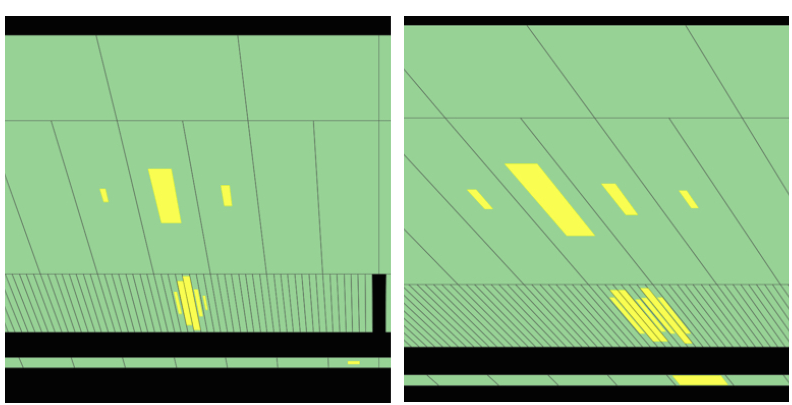
\includegraphics[width=0.7\linewidth]{4_photonid/shower_shapes/PhotonPizero}
    \caption{Characteristic energy deposits by an isolated photon (left), and a \(\pizero\to\gamma\gamma\) event (right), which is possible to distinguish thanks to the granularity of the first \ac{ECAL} layer~\cite{ATLAS-ECAL-Pizero}.}
    \label{fig:pid_ss:ss:pizero}
\end{figure}






\section{Photon Identification}


\subsection{Optimisation}
\label{subsec:pid_ss:pid:optimisation}

Starting from these discriminating \acp{SSV}, three \acp{WP} can be defined: \textit{loose}, \textit{medium} and \textit{tight} \acp{WP}~\cite{ATLAS-EGamma-Performance-2024}. The loose \ac{WP} is employs cuts to the variables defined in the second layer and to the hadronic leakage variable, used primarily by the trigger. The medimum \ac{WP} is a \ac{WP} optimised to have a flat \(95\%\) efficiency. This \ac{WP} applies cut to all the previously defined variables (strip and middle layer and leaks to the \ac{HCAL}). Finally, the tight \ac{WP}, uses all the \acp{SSV} defined and provides an excellent background rejection. TABLE shows which variables are used for each \ac{WP}.

ADD PLOTS OF ALL THE VARIABLES COMPARING REAL AND FAKE

The cuts on the \acp{SSV} for each identification \ac{WP} are optimised as a function of the transverse energy and the pseudo-rapidity of the photon candidate, to account for the shape of the variables for different \(\eta\) and for variations in the amount of material and the geometry of the calorimeter. The three \acp{WP} are also optimised separately for converted and unconverted photons.
The optimisation is performed with a \ac{MV} approach where signal efficiencies are scanned between \(0\%\) and \(100\%\) while trying to maximise the background rejection. The resulting, optimised, cut values are subject to fluctuations and therefore they are manually smoothed.

Two different \ac{MC} samples are used for the optimisation procedure, representative at different \ptgam. For photons with \(10<\pt<25~\gev\), radiative \Zboson decays (\(\Zboson\to\ellell\gamma\)) samples are used as signal, while \Zjets events accounts for the background. Events used are selected by requiring two opposite charged leptons and a minimum angular separation between the photon and the lepton of \(\DeltaR_{\text{min}}(\ell, \gamma) > 0.4\). To reject non-radiating \Zboson bosons, the dilepton invariant mass has to satisfy \(m_{\ell\ell}<83~\gev\), and the three-body invariant mass \(m_{\gamma\ell\ell}\) needs to approximate the \Zboson boson mass: \(80~\gev < m_{\gamma\ell\ell} < 100~\gev\). Finally, the photon is required to have \(\abseta<2.37\), excluding the crack region.
Finally, for higher \pt photons, \(\pt>25~\gev\), the inclusive-photon (\yj) signal events are compared agains dijet backgrounds. The event selection used in this case is simply requiring the photon to be in the \ac{ECAL} acceptance region (excluding the crack).





\subsection{Efficiency measurements}

Photon identification efficiency measurements are carried out using three different methods that are detailed in \Refn{\cite{ATLAS-EGamma-Performance-2015-2016}} and that are combined to yield correction factors for analyses. In all cases, photons are required to satisfy the Loose isolation criterion defined in \Refn{\cite{ATLAS-EGamma-Performance-2015-2016}} and therefore the photon efficiencies are measured relative to this isolation criterion. In the following paragraphs, a brief description of each method is given.

For the lower \pt range (\(7<\pt<100~\gev\)), photons from radiative \Zboson decays are used as signal photons, selecting the events in the same way as for the \acp{WP} optimisation (\Sect{\ref{subsec:pid_ss:pid:optimisation}}). The only difference in this case, is an additional lower limit on the di-lepton invariant mass of \(40<m_{\ellell} < 83~\gev\). To estimate the number of signal and background events, template fits to the observed three-body invariant-mass distribution are performed.

The second method to compute efficiencies relies on Smirnov transformations~\cite{SmirnovTransform} to the electrons' \acp{SS} to resemble those of photons'. The samples used in this approach are \(\Zboson\to ee\) decays, in which the electrons are required to pass loose photon isolation. The candidate electrons in data contain a small background from \Wjets and multijet production; this background is subtracted by fitting simulated signal samples and background templates derived from data control regions to the \(m_{ee}\) data distributions. The electron candidates are counted for events in the range \(70 < m_{ee} < 110~\gev\), and the efficiencies are measured using the tag-and-probe method described in \Refn{\cite{ATLAS-EGamma-Performance-2015-2017}}. The \pt range in which this method is implemented is \(25<\pt<250~\gev\).

The final and third method uses higher \pt photons originating from \ac{QCD} \gammajet production with transverse momenta in the range \(50<\pt<1500~\gev\). The photons for this study are required to pass the loose identification \ac{WP} employed in the trigger. This sample is dominated by background dijet events whose production cross section is orders of magnitude higher. The maxtrix method~\cite{ATLAS-EGamma-Performance-2015-2016} is used in this case, which constructs four orthogonal regions that either pass or fail the tight identification \ac{WP}, and pass or fail the track-isolation (described in \Sect{\ref{subsec:objects:egamma:iso}}). For each region, two unknowns arise: the number of signal and background events.
If the track isolation efficiencies are known for the signal and background components, then it is possible to estimate the efficiency for loose photons passing the tight identification criteria. The isolation efficiencies for signal photons are estimated using \ac{MC} samples, and the ones for backgrounds are obtained in a jet-enriched control region constructed by inverting the identification criteria.
The efficiency measurements in data for the tight identification \ac{WP} then reads:
\begin{equation}
    \varepsilon^{\text{tight-ID}} = \frac{
        \frac{
            \hat{\varepsilon}_{\text{ID}} - \hat{\varepsilon}_{\text{ID}}^b
        }{
            \hat{\varepsilon}_{\text{ID}}^s - \hat{\varepsilon}_{\text{ID}}^b
        }
        \cdot
        N_{\text{ID}}^T
    }{
        \frac{
            \hat{\varepsilon} - \hat{\varepsilon}^b
        }{
            \hat{\varepsilon}^s - \hat{\varepsilon}^b
        }
        \cdot
        N^T
    },
\end{equation}
where \(N^T\) accounts for the totality of photons in the inclusive sample which consists on \(N^s\) prompt photons (or signal photons) and \(N^b\) fake photons (background photons). The number \(N^T_{\text{ID}}\) is the subset of \(N^T\) that pass the identification requirement. Data, signal and background track isolation efficiencies are represented by \(\hat{\varepsilon}\), \(\hat{\varepsilon}^s\) and \(\hat{\varepsilon}^b\), respectively. Similarly, the track isolation efficiencies for those photons passing tight identification are shown as \(\hat{\varepsilon}_{\text{ID}}\), \(\hat{\varepsilon}_{\text{ID}}^s\) and \(\hat{\varepsilon}_{\text{ID}}^b\), respectively. The measured efficiencies for photons with \(\pt>150~\gev\) is between \(90\) and \(96\%\).

Since data and simulation measured efficiencies do not match, \ac{MC} needs to be corrected to account for these differences. In the ideal case where one expects perfect agreement between both samples, ratios of the data efficiencies to simulation efficiencies in each \(\pt-\eta\)-conversion status bin should be \(1.0\). These ratios are referred as \acp{SF} and are computed separately for each one of the methods described. Then, the different methods' \acp{SF} are combined using a weighted average in each bin, assuming the statistical and systematic uncertinaties to be uncorrelated between the methods. Resulting \acp{SF} in all cases are consistent with \(1.0\), only deviating by a maximum of \(2\%\). The only exception to this case is in the first \pt-bin (\(7<\pt<10~\gev\)) where deviations of up to \(30\%\) take place.





\section{Shower shapes variables differences between data and MC}

The \ac{ATLAS} \ac{MC} simulation does not perfectly describes data. This is clearly seen when computing the previsously mentioned \acp{SF}, whose values were different from 1, meaning that different efficiencies are obtained in data and in \ac{MC}. In particular, when comparing the \acp{SS} distributions, it is seen that \ac{MC} distributions are shifted or even the whole shape differs.

The main differences on the distributions arise for the \(\eta\) shower profiles, where broader distributions were seen in data compared to \ac{MC}. Part of the effect was corrected in 2010 after moving to detailed description of the material composition in the accordion absorbers in \textsc{Geant4}. However, the remaining data-\ac{MC} disagreements are still under study and could be due to several potential effects:
\begin{itemize}
    \item Detector geometry description of the lead thickness (including possible variations of due to gravity) or material composition, material before the \ac{ECAL}, a decrease of the width of cells caused by calorimeter contraction due to temperature (mainly in the first layer).
    \item Mismodeling of the electric field in the \ac{LAr} gaps.
    \item Mismodeling of the cross-talk effect (energy sharing between calorimeter cells due to electronics possible in \(\eta\) direction).
\end{itemize}



To account for the differences in the \acp{SS}, historically, corrections were made in the form of shifts to each one of the \ac{MC} distributions. These shifts comprised the so-called \acp{FF}, and were determined using a \chisq minimisation on the comparison of data and \ac{MC} \acp{SS}~\cite{ATLAS-EGamma-Performance-2015-2016,ATLAS-EGamma-Performance-2015-2017}.
Even though the differences decreased substantially after these corrections, some of them remained, shown in FIGURE. It is seen from the distributions that the main differences that remained are related to the shape of the distributions, therefore needing for higher order corrections. In \Ch{\ref{ch:ffs}} a detailed description of newly derived corrections is presented.
Since \acp{SS} are built from energy deposits on the \ac{ECAL} cells, another possible way of correcting the current disagreement between data and \ac{MC} \acp{SS} is to directly correct the energies on \ac{MC} at a cell-level, fixing the differences in all \acp{SSV} at once. This new approach is studied in \Ch{\ref{ch:cellrw}}.


\section{Samples and event selection for the \ac{SS} correction studies}

As mentioned above, the improved \ac{FF} method and a novel cell-based reweighting method is presented in \Chs{\ref{ch:ffs}}{\ref{ch:cellrw}}.

Similar to what had been done for the identification optimisation studies, two photon samples are used for the \acp{FF} calculation. For photons with \(7\leq\ptgam\leq 50~\gev\), \ac{FSR} photons from \Zboson-boson decay are considered, while photons from \ac{QCD} \gammajet events are used for photons with \(\ptgam\geq50~\gev\), hereinafter referred as \ac{RZ} photons and \ac{SP} samples, respectively. On the other hand, for the cell-level corrections to the \acp{SSV}, only \ac{RZ} photons are used. In what follows, event selection for both types of samples is detailed.

For both types of corrections, the \ac{MC} samples are reweighted to match the luminosity of the collected \ac{ATLAS} data, and also pileup re-weighted to match the pileup profile shown in \Sect{\ref{sec:atlas:runs}}.

\subsection{Radiative \Zboson boson decays}

For low-\pt photons, \ac{RZ} photons are used as signal photons, while backgrounds are modeled by \(\Zboson\to\ell\ell\) events. The photons are required to pass the following selection:
\begin{itemize}
    \item \textbf{\ac{ECAL} \abseta acceptance region}. First of all, the photons are required to be inside the \ac{ECAL} acceptance region excluding the crack, detailed in \Sect{\ref{subsubsec:atlas:atlas:cals:ecal}}, given by \(\abseta<1.37\) or \(1.52<\abseta<2.37\). 
    \item \textbf{Isolation}. Fake photon candidates are removed by imposing an isolation requirement on the calorimetric isolation variable with the \texttt{FixedCutTightCaloOnly} \ac{WP}.
    \item \textbf{\ac{FSR} selection}. As shown in FIGURE, the vast majority of events correspond to \(m_{\gamma\ell\ell}>100~\gev\) and \(m_{\ell\ell}\sim m_{\Zboson} \approx 91~\gev\), which represent \ac{ISR} photons (photons radiated from the inital quarks). Photon candidates from \ac{ISR} are largely affected by the \Zjets background, where a jet fakes a photon~\footnote{The production cross-section of \Zjets is about three orders of magnitude higher than that of \(\Zboson+\gamma\), and a non-negligible fraction of jets contains high-\pt \pizero's, decaying to collimated photon pairs}.
    However, a second peak appears in the distribution where the three-body invariant mass approximates the \Zboson mass (\(m_{\gamma\ell\ell}\approx m_{\Zboson}\)). These particular type of events are referred as \ac{FSR} photons, characterised by high real photon purity, and are the ones of interest for the correction studies.
    \item \textbf{Photon-lepton overlap}. By requiring a minimum angular distance between the photon and the closest lepton (\(\DeltaR_{\text{min}}>0.4\)), biases in the \ac{ECAL} deposits by the objects are avoided.
    \item \textbf{Truth-matching}. \fixme{give description here}
\end{itemize}


\subsubsection{Special selection for cell-based reweighting corrections}

For the cell-energy reweighting method to correct the \acp{SS}, a special selection needs to be applied to the \ac{EM} clusters. For the current studies, only \acp{SS} built from the second layer are studied. Clusters of \(7\times 11\) cells in \(\eta\times\phi\) are considered, shown in FIGURE with the current cell arrangement used.

In this work, only "healthy clusters" are considered, that is, events need to be associated to clusters of 77 cells (no cells missing) and the central cell must be the one with highest energy in the corresponding cluster ("hottest" cell). In FIGURE, an example of the averaged energies at each cell, for events with unconverted photons in data is shown.

For these particular studies, the photon isolation requirement is relaxed to the \texttt{FixedCutLoose} \ac{WP} is used.

%  and no identification selection is applied. The same \ac{FSR} requirements are posed on the events in which the invariant masses must satisfy \(80 < m_{\gamma\ell\ell} < 100~\gev\) and \(40<m_{\ellell} < 83~\gev\) which removes the majority of non-\ac{FSR} photons. The photon to the closest lepton candidate are required to be separated by a minimum angular distance of \(\DeltaR_{\text{min}}>0.4\), and the photons need to be in the \ac{ECAL} acceptance region of 

\subsection{Inclusive photons}

Photon+jet events are used for the high-\pt regime of the \acp{FF} corrections. The events pass loose identification trigger requirements and for the nominal values of the corrections tight identification is applied. This selection is applied to reduce the vast di-jet background, which has much higher production cross-sections. As for the \ac{RZ} photon samples, the photons are required to be within the \ac{ECAL} acceptance region excluding the crack.